\insertdesignoverview{Glyph Arm}
{Collect and deliver glyphs without having to turn around; Control the placement of the glyphs} % Goals of the mechanism
{arm_good.png}% CAD Image
{arm_build.jpg}% Build Image
{0.25" Medium Density Fiberboard, 5mm Underlayment, 0.22" Delrin, Aluminum, ABS Plastic, Steel Linear Bearings}% Materials ex. 0.25" MDF, Aluminum, etc
{Laser Cutting, 3D Printing, Lathe work, CNC Milling, Surface Grinding}% Manufacturing Processes ex. Laser Cut, 3D print, etc.


\interesting{Our innovative glyph delivery mechanism, analyzed in depth}{Innovate:55}


\subsection*{How it Works}
Two claws move down and grab two glyphs sitting on the intake tray. A 60:1 Neverrest motor rotates the arm and claw, moving the glyphs to the top of the back wall. Two independent belts move each claw over so that the glyphs are in between the column structures of the cryptobox. Then the claws release the glyphs and they fall down to the top of their respective stacks.

\subsection*{Claw}
When we designed the Claw in Creo, we used a sophisticated technique called motion skeletons. This allowed us to define the geometry and joints of the claw with sketchs. We could then simulate the movement within the motion skeleton. From there we could build our parts around the skeleton, and attach them to the moving bodies.

\begin{figure}[htp]
\centering
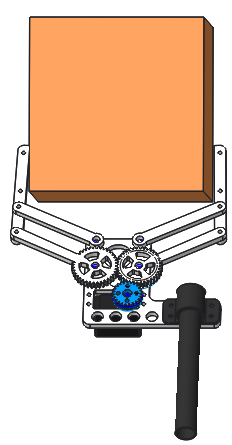
\includegraphics[width=.3\linewidth]{Design_Overview/arm_claw.png}
\caption{Claw Assembly}
\label{fig:arm_claw}
\end{figure}

\subsection*{Iterations}
The axis of rotation on our first arm design was farther from the middle and closer to the ground. This made the blocks fall back into the robot when we tried to drop them over the top of the back wall. To fix this, we moved the axis of rotation further up and closer to the center plane. 

\subsection*{Sensors and Control}
We have two external encoders attached to the belts of the arm sliders. This allows us to move the claws to specific locations. We created functions that move the two arms in sync with the joysticks, and move them the correct spacing to score into the cryptobox.

We have a PID control algorithm that uses all the constants of PID to control the rotation of the arm. The force required to rotate the arm changes with position due to the effects of gravity. When the arm is rotating up, it requires torque to lift the glyphs, though when it passes the vertical plane, it requires less power as gravity is working in the same direction to bring it down. The PID algorithm acts as a feedback loop, accounting for those changes.

\interesting{The effects of gravity on our rotating glyph delivery arm}{Design:45}
\begin{figure}[htp]
\centering
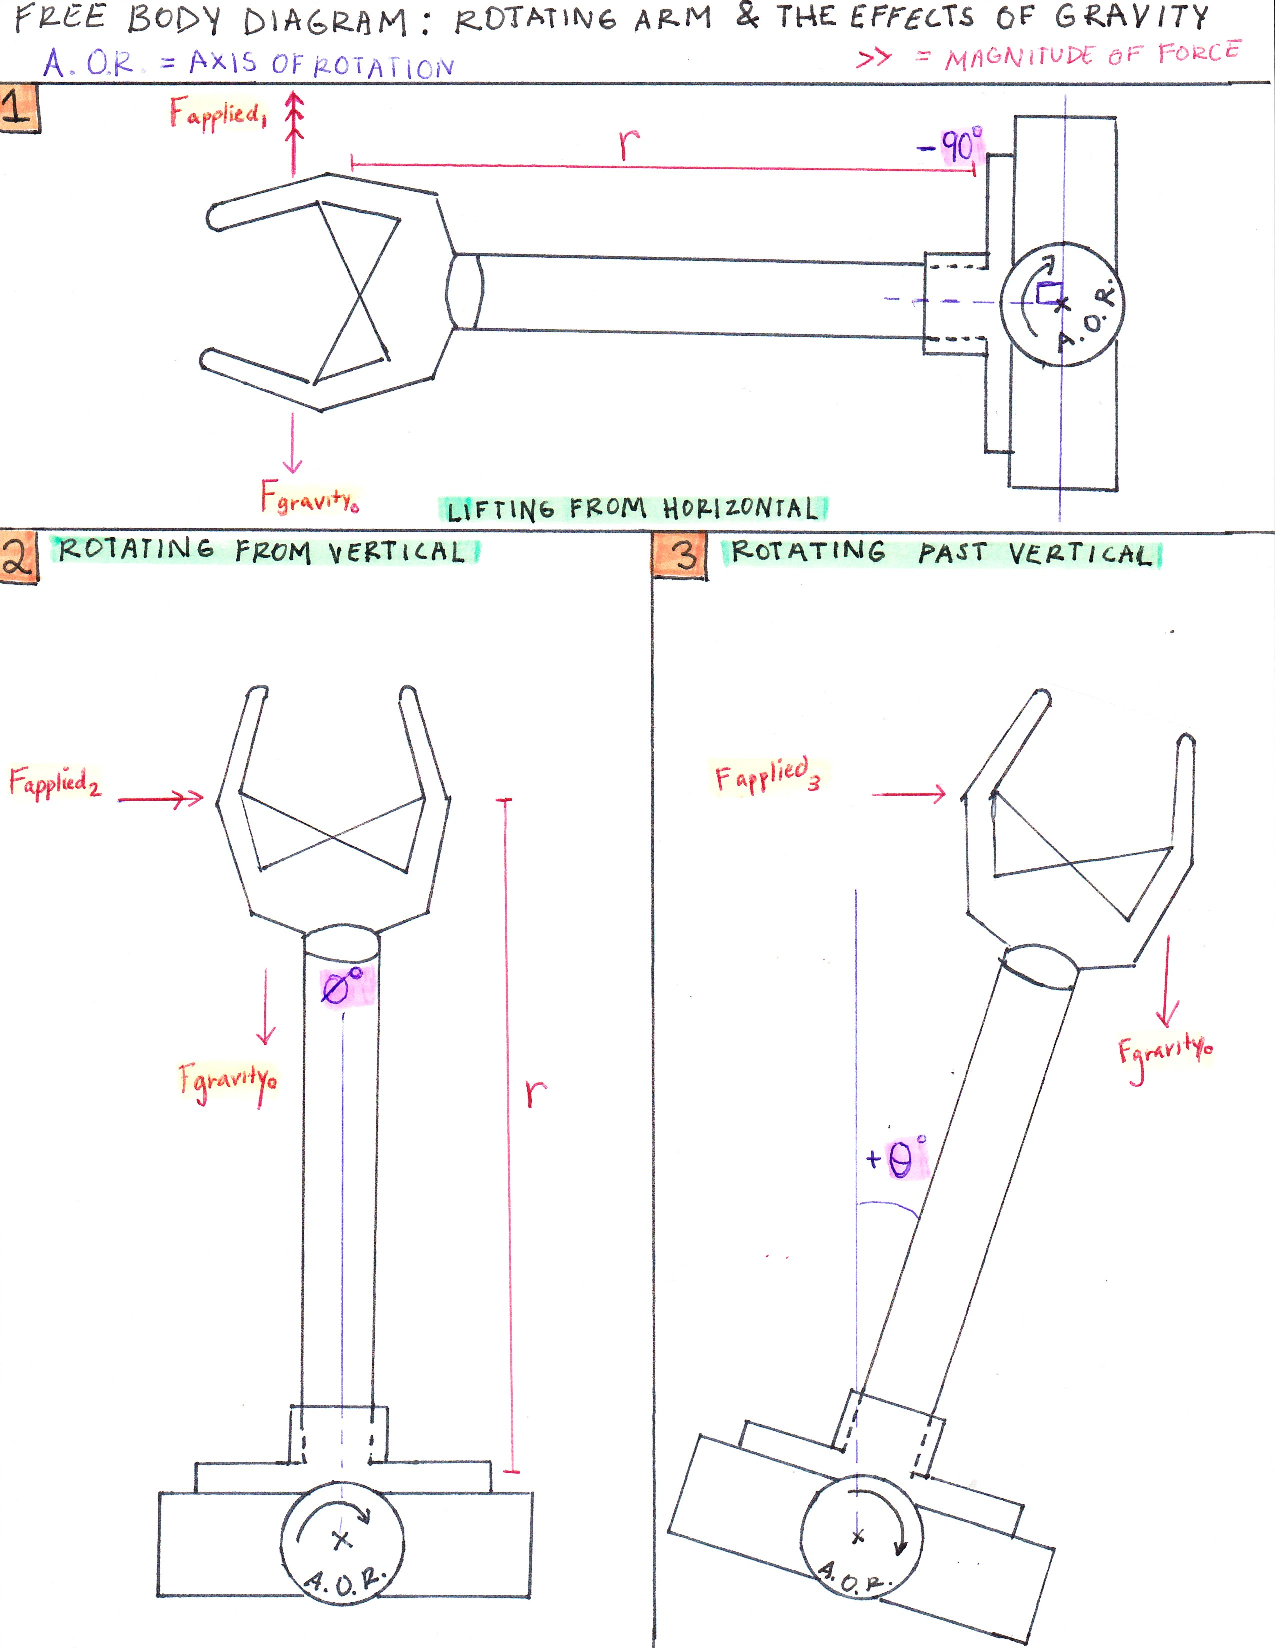
\includegraphics[width=.7\linewidth]{Design_Overview/FBD_good_arm.pdf}
\caption{Free Body Diagram at Different Arm Positions}
\label{fig:FBD_Arm}
\end{figure}


\vskip 0.25in
Rotating Arm and the Effects of Gravity:
\vskip 0.05in
\textit{
\\The goal is to keep the angular acceleration of the arm constant by changing the force applied. 
\\These equations go with the Free Body Diagram of the arm.
\\The arm starts out in the horizontal plane and rotates clockwise. 
\\Angles are measured from the vertical plane.
}
\vskip 0.1in
\interesting{Detailed equations depict the effect of gravity on the arms}{Think:22}
\textit{
\\Fgravity = Weight of Arm
\\Fapplied = Force to rotate arm
\\A.O.R. is the Axis of Rotation
\\r = Distance from A.O.R. to Claw
}

\vskip 0.2in
Base Equations:
\[\tau = m\alpha\]
\[\tau = F*r\]
\[(Fapplied + Fgravity*sin\theta)r = m\alpha\]

At Position 1, \[\theta = -90 degrees\]
\[(Fapplied_{1} + Fgravity*sin(-90))r = m\alpha\]
\[(Fapplied_{1} - Fgravity)r = m\alpha\]

At Position 2, \[\theta = 0 degrees\]
\[(Fapplied_{2} + Fgravity*sin(0))r = m\alpha\]
\[(Fapplied_{2})r = m\alpha\]

At Position 3, \[\theta \geq 0 degrees\]
\[(Fapplied_{3} + Fgravity*sin(+\theta))r = m\alpha\]

\subsection*{Equation Analysis}
\textit{
\\The force applied at position 1 must be the greatest of the three positions because the force of gravity is working against it. The force applied in position 2 can be less because it is working perpindicular to the force of gravity. The force applied in position 3 should be the least because a component of the force of gravity is working in the same direction to bring the arm down.
}

\subsection*{Mechanism Accomplishments}
\begin{itemize}
    \item It can place the glyphs in any column, giving us more flexibility to complete the cryptokey
    \item It grabs the glyphs in the front and places them in the back, so that we don't waste time turning around between cycles
    \item It drops the glyphs from the top so we don't have to worry about placing the blocks in specific rows.
\end{itemize} 